% !TeX document-id = {d0a1af33-8d18-4143-aea1-eb0b4e8d785e}
% !TeX encoding = UTF-8
% !TeX TXS-program:compile =txs:///pdflatex/[--shell-escape]| txs:///makeglossaries| txs:///pdflatex/[--shell-escape]


%%%%%%%%%%%%%%%%%%%%%%%%%%%%%%%%%%%%%%%%%%%%%%%%%%%%%%%%%%%%%%
%
%  Allgemeine Kommentare
%
%%%%%%%%%%%%%%%%%%%%%%%%%%%%%%%%%%%%%%%%%%%%%%%%%%%%%%%%%%%%%%
%Dieses Dokument ist für die Verwendung von pdf-latex geschrieben. Dies muss für die Kompilierung beachtet werden. Falls das normal Latex verwendet werden soll, müssen die Bilder in ps/eps Format vorliegen. 

%Beim Anlegen von großen Dokumenten bietet es sich an, nicht alles in eine Datei zu schreiben. Latex bietet hier die Möglichkeit einzelne Dateien durch \input{Dateiname.tex} einzubinden. Man kann also für z.B. jedes Kapitel eine eigene Datei schreiben. In diese Datei gehört aber nicht der ganze Vorspann (Definition von packages etc...). Hierdurch ist es auch einfach möglich nur Teile der großen Arbeit anzusehen, indem man die anderen \input Befehle auskommentiert. Für jedes Kapitel sollte eine eigene Texdatei angelegt werden, die in "gliederung.tex" mit eingebunden werden.

%Häufig möchte man nur schnell seine Änderungen im Dokument ansehen, aber das Kompilieren dauert wegen der vielen Bilder sehr lange. Hier kann man ganz oben in die documentclass als weitere Option draft einfügen. Dann werden anstatt der Bilder nur Kästen im Dokument erzeugt und das Kompilieren geht sehr viel schneller. 

%Es ist sehr wichtig darauf zu achten Absätze und leere Zeilen geeignet zu verwenden. Wenn ein Absatz gewünscht ist, muss eine leere Zeile im tex Dokument erzeugt werden, welche nicht mit \\ abgesetzt wird! Ansonsten muss auf leere Zeilen verzichtet werden, da diese sonst zusätzliche freie Räume erzeugen. Vor allem beim Schreiben von Formeln sind leere Zeilen wegen der Übersicht häufig eingefügt. Diese müssen entfernt oder durch ein % auskommentiert werden. Ähnliches ist beim Einbinden von Figures zu beachten. 

%Für Literaturreferenzen können wir euch die Programme JabRef oder Citavi empfehlen. Dort kann man sehr einfach die einzelnen Einträge machen und die dadurch entstandene Bibliothek einbinden. 

%Als Editor für die Arbeit mit Tex hat sich Texstudio bei uns etabliert. Ein großer Vorteil ist, dass man den Tex Code und das eigentliche Dokument nach der Kompilierung nebeneinander sieht und es lassen sich auch sonst noch viele nette Sachen einstellen. Zum Beispiel versteht TexStudio sogenannte Magic-Comments, die den Compiler-Aufruf und die Dateikodierung festlegen lassen. Beim ersten Kompilieren ist der Vertrauenabfrage des Editors zuzustimmen. Für die Verwendung des Befehls "makeglossaries", welcher eine sehr einfache Generierung der Abkürzungs- und Symbolverzeichnisse ermöglicht, muss Perl (z.B. activeperl) installiert sein. Alle genannten Programme kann man kostenlos im Internet erhalten (Citavi über die Bibo).

%Der Benutzer der Vorlage muss ausschließlich folgende Dateien bearbeiten:
%myData.tex
%abstract_de.tex
%abstract_en.tex
%gliederung.tex
%einleitung.tex 
%kapitel_xy.tex (alle Kapitel)
%notation.tex
%anhang.tex


%Viel Vergnügen beim Schreiben Eurer Dissertation wünschen,
%Martin, Julia, Christopher und Phillip
%Bei Fragen wende dich bitte an: redaktion@hni.upb.de


%%%%%%%%%%%%%%%%%%%%%%%%%%%%%%%%%%%%%%%%%%%%%%%%%%%%%%%%%%%%%%
%  Einstellungen
%%%%%%%%%%%%%%%%%%%%%%%%%%%%%%%%%%%%%%%%%%%%%%%%%%%%%%%%%%%%%%

% !TeX encoding = UTF-8
\documentclass[a4paper,twoside,12pt,ngerman,openright,titlepage,halfparskip,headings=small,bibtotoc,pointlessnumbers,fleqn]{scrreprt} %[optionen]{Klasse}
%[..,zweiseitig,..,neue dt.Rechtschr.,chaptereröffnung nur auf ungeraden Seiten,mit Titelseite, halbe Leerzeile bei Absätzen,
% ..,kleine Überschriften,Literaturverzeichniseintrag ins Inhaltsverzeichnis,keine Punkte hinter chapternummern]

%%%%%%%%%%%%%%%%%%%%%%%%%%%%%%%%%%%%%%%%%%%%%%%%%%%%%%%%%%%%%%
% Packages
%%%%%%%%%%%%%%%%%%%%%%%%%%%%%%%%%%%%%%%%%%%%%%%%%%%%%%%%%%%%%%
\usepackage{emptypage}
\usepackage[utf8]{inputenc}
\usepackage[ngerman]{babel}										%neue deutsche Rechtschreibung
\usepackage[T1]{fontenc}
\usepackage[scaled]{uarial} 									%T1 Schriftsatz
\usepackage{hyperref}
\usepackage{graphicx}											%Einfügen von Bildern
\usepackage[left=3cm,right=3.0cm,top=1.25cm,bottom=1.25cm,includeheadfoot]{geometry}	%Seitenaufteilung
\usepackage{tabularx,array,booktabs,calc,multirow}				% Tabellen
\usepackage{mathcomp}
\usepackage{cite}
\usepackage{pdfpages}											% Einbindung von PDFs
\usepackage[babel,german=quotes]{csquotes}
\usepackage[font={normalsize,it}]{caption}
\usepackage{subcaption}										% Bei Bildern nebeneinander einzelne Bildunterschriften
\usepackage{xcolor}
\usepackage{textcomp}
\usepackage{paralist}											% Erweiterte Aufzählungsmöglichkeiten
\usepackage{xifthen}											% ifempty

%%%%%%%%%%%%%%%%%%%%%%%%%%%%%%%%%%%%%%%%%%%%%%%%%%%%%%%%%%%%%%
% Mathe-Pakete
%%%%%%%%%%%%%%%%%%%%%%%%%%%%%%%%%%%%%%%%%%%%%%%%%%%%%%%%%%%%%%
\usepackage{amsfonts}
\usepackage{amsmath}
\usepackage{amssymb}											% Symbole für Zahlenmengen usw.
\usepackage{cancel}												% Terme durchstreichen


%%%%%%%%%%%%%%%%%%%%%%%%%%%%%%%%%%%%%%%%%%%%%%%%%%%%%%%%%%%%%%
% Schriftart
%%%%%%%%%%%%%%%%%%%%%%%%%%%%%%%%%%%%%%%%%%%%%%%%%%%%%%%%%%%%%%
\usepackage{txfonts} 											% Schrift Times
 
%%%%%%%%%%%%%%%%%%%%%%%%%%%%%%%%%%%%%%%%%%%%%%%%%%%%%%%%%%%%%%
% Koma-Style
%%%%%%%%%%%%%%%%%%%%%%%%%%%%%%%%%%%%%%%%%%%%%%%%%%%%%%%%%%%%%%
\usepackage{scrpage2}
	% Kopfzeile
	\pagestyle{scrheadings} 									% eigener Seitenstil
	\clearscrheadings											% alle Voreinstellungen löschen
	\ohead{\pagemark}											% Seitenzahl oben außen
	\automark[chapter]{chapter} 								% \headmark definieren als Kapitelname
	\renewcommand{\chapterpagestyle}{scrheadings}				% Kapitelbeginn wie der Rest
	\rehead{\chaptername~\thechapter}							% Kapitelnummer   	
	\renewcommand{\chaptermark}[1]{\markright{#1}}	
	\lohead{\headmark}											% Kapitelname links auf ungeraden Seiten
	\lefoot{}\refoot{}\lofoot{}\rofoot{}\cehead{}\cohead{}		% keine Seitenzahlen in Fußzeilen
	\setheadsepline{0.2pt}										% Trennlinie zwischen Kopf und Textkörper
	\addtokomafont{pagehead}{\footnotesize}						% Schrift in Kopfzeile um einen Faktor kleiner als Standard
	\addtokomafont{pagehead}{\upshape}							% Schrift in Kopfzeile aufrecht (nicht kursiv)
	\addtokomafont{footnote}{\sffamily}							% Fußnoten serifenlos

%%%%%%%%%%%%%%%%%%%%%%%%%%%%%%%%%%%%%%%%%%%%%%%%%%%%%%%%%%%%%%
% Gestaltung der Überschriften
%%%%%%%%%%%%%%%%%%%%%%%%%%%%%%%%%%%%%%%%%%%%%%%%%%%%%%%%%%%%%%
	\parindent0cm																							
	\parskip\medskipamount	
	\renewcommand*{\chapterformat}{%
		\makebox[1.5cm][l]{\chapappifchapterprefix{\ }\thechapter\autodot\enskip}} 	% Chapter exakt 1.5cm hängend
	\renewcommand*{\othersectionlevelsformat}[1]{%
		\makebox[1.5cm][l]{\csname the#1\endcsname\autodot\enskip}}					% Section und Subsection hängend
	
	\RedeclareSectionCommand[
	beforeskip=-24pt,																%Abstand vor Chapter
	afterskip=12pt,																	%Abstand nach Chapter
	font=\bfseries\fontsize{14}{1.5\baselineskip}\selectfont]{chapter}				%Schriftgröße und Zeilenabstand
	
	\RedeclareSectionCommand[
	beforeskip=-24pt,
	afterskip=8pt,
	font=\bfseries\fontsize{13}{16}\selectfont]{section}
	
	\RedeclareSectionCommand[
	beforeskip=-24pt,
	afterskip=8pt,
	font=\bfseries\fontsize{12}{16}\selectfont ]{subsection}

%%%%%%%%%%%%%%%%%%%%%%%%%%%%%%%%%%%%%%%%%%%%%%%%%%%%%%%%%%%%%%
% Zahlen und Einheiten SIUNITX
%%%%%%%%%%%%%%%%%%%%%%%%%%%%%%%%%%%%%%%%%%%%%%%%%%%%%%%%%%%%%%
\usepackage{siunitx}								% Zahlen + Einheiten Bsp:\SI{9.81}{\meter\per\square\second}
	\sisetup{output-decimal-marker = {,}}
	\DeclareSIUnit[number-unit-product = \,] 
	\U{U}
	\DeclareSIUnit[number-unit-product = \,] 
	\Umin{\U \per \minute}
	\DeclareSIUnit[number-unit-product = \,] 
	\Us{\U \per \s}
	\DeclareSIUnit[number-unit-product = \,] 
	\Uss{\U \per \square\s}
	\DeclareSIUnit[number-unit-product = \,] 
	\decade{dek}

%%%%%%%%%%%%%%%%%%%%%%%%%%%%%%%%%%%%%%%%%%%%%%%%%%%%%%%%%%%%%%
% Befehl \vec für Vektorunterstriche
%%%%%%%%%%%%%%%%%%%%%%%%%%%%%%%%%%%%%%%%%%%%%%%%%%%%%%%%%%%%%%
\usepackage{accents}											% für Vektorunterstriche
	\renewcommand{\vec}[1]{\underaccent{\bar}{#1}}

%%%%%%%%%%%%%%%%%%%%%%%%%%%%%%%%%%%%%%%%%%%%%%%%%%%%%%%%%%%%%%
% Quellcode-Listing Einstellungen
%%%%%%%%%%%%%%%%%%%%%%%%%%%%%%%%%%%%%%%%%%%%%%%%%%%%%%%%%%%%%%
\usepackage{color,listings}
\usepackage{matlab-prettifier}
	\lstset{numbers=left, numberstyle=\tiny,language=[Sharp]C,showspaces=false, showstringspaces=false, breaklines=true,captionpos=b, tabsize=2}
	\lstset{literate=%
		{Ö}{{\"O}}1
		{Ä}{{\"A}}1
		{Ü}{{\"U}}1
		{ß}{{\ss}}1
		{ü}{{\"u}}1
		{ä}{{\"a}}1
		{ö}{{\"o}}1
		{~}{{\textasciitilde}}1
	}
	
	\definecolor{latexkeyword}{RGB}{0,149,255}
	\definecolor{codegray}{rgb}{0.5,0.5,0.5}
	
	\lstdefinestyle{myLatexStyle}{
		language=[LaTeX]TeX,
		frame=single,
		backgroundcolor=\color{white},
		rulecolor=\color{lightgray!40},
		breaklines=true,
		%  xleftmargin=\parindent,
		basicstyle=\footnotesize\ttfamily,
		keywordstyle=\bfseries\color{purple!40!black},
		commentstyle=\itshape\color{green!40!black},
		%identifierstyle=\color{blue},
		stringstyle=\color{orange}}

%%%%%%%%%%%%%%%%%%%%%%%%%%%%%%%%%%%%%%%%%%%%%%%%%%%%%%%%%%%%%%
% Eigene Environments
%%%%%%%%%%%%%%%%%%%%%%%%%%%%%%%%%%%%%%%%%%%%%%%%%%%%%%%%%%%%%%
\usepackage{environ}											% Neue Environments siehe Settings
	\NewEnviron{es}
	{
		\begin{equation}
		\begin{split}
		\BODY
		\end{split}
		\end{equation}
	}
	
	\NewEnviron{es*}
	{
		\begin{equation*}
			\begin{split}
				\BODY
			\end{split}
		\end{equation*}
	}
%%%%%%%%%%%%%%%%%%%%%%%%%%%%%%%%%%%%%%%%%%%%%%%%%%%%%%%%%%%%%%
% Mathtools Settings
%%%%%%%%%%%%%%%%%%%%%%%%%%%%%%%%%%%%%%%%%%%%%%%%%%%%%%%%%%%%%%
\usepackage{mathtools}											% Nummerierung von referenzierten Gleichungen
	\mathtoolsset{showonlyrefs} %Nur Gleichungen die mit \eqref{label} referenziert werden nummerieren (mathtools)


%%%%%%%%%%%%%%%%%%%%%%%%%%%%%%%%%%%%%%%%%%%%%%%%%%%%%%%%%%%%%%
% Nomenklatur
%%%%%%%%%%%%%%%%%%%%%%%%%%%%%%%%%%%%%%%%%%%%%%%%%%%%%%%%%%%%%%
\usepackage[acronym,nonumberlist,nomain]{glossaries} %Paket glossaries
\usepackage{glossary-super} %besonderer style, den ich gut finde 

\setlength{\glsdescwidth}{15cm}

\newglossary[slg]{symbolslist}{syi}{syg}{Symbolverzeichnis} % create add. symbolslist


\glsaddkey{unit}{\glsentrytext{\glslabel}}{\glsentryunit}{\GLsentryunit}{\glsunit}{\Glsunit}{\GLSunit}
\makeglossaries                                   % activate glossaries-package

\glssetnoexpandfield{unit}
\glsdisablehyper
\newglossarystyle{symbunitlong}{%
	\setglossarystyle{long3col}% base this style on the list style
	\renewenvironment{theglossary}{% Change the table type --> 3 columns
		\begin{longtable}{lp{0.7\glsdescwidth}>{\centering\arraybackslash}p{2cm}}}%
		{\end{longtable}}%
	%
	\renewcommand*{\glossaryheader}{%  Change the table header
		\bfseries Name & \bfseries Beschreibung & \bfseries Einheit \\
		\hline
		\endhead}
	\renewcommand*{\glossentry}[2]{%  Change the displayed items
		\glstarget{##1}{\glossentryname{##1}} %
		& \glossentrydesc{##1}% Description
		& $\left[\glsunit{##1}\right]$  \tabularnewline
	}
}

%%%%%%%%%%%%%%%%%%%%%%%%%%%%%%%%%%%%%%%%%%%%%%%%%%%%%%%%%%%%%%
% Inhaltsverzeichnis
%%%%%%%%%%%%%%%%%%%%%%%%%%%%%%%%%%%%%%%%%%%%%%%%%%%%%%%%%%%%%%
\usepackage{tocstyle}
\newtocstyle[KOMAlike][leaders]{alldotted}{}
\usetocstyle{alldotted}
\addtotoclist{toa} %Table of Appendix
\newcounter{appendix}[chapter]
\renewcommand{\theappendix}{\thechapter.\arabic{appendix}}

%%%%%%%%%%%%%%%%%%%%%%%%%%%%%%%%%%%%%%%%%%%%%%%%%%%%%%%%%%%%%%
% Plots aus Matlab mit pgfplots
%%%%%%%%%%%%%%%%%%%%%%%%%%%%%%%%%%%%%%%%%%%%%%%%%%%%%%%%%%%%%%
\usepackage{pgfplots}
\pgfplotsset{every axis/.append style={		
		ticklabel style={/pgf/number format/.cd, use comma, 1000 sep = {},fixed,precision=2}		
	}
}
\pgfplotsset{%
	every axis plot post/.append style={line width = 2pt}} 
%\pgfplotsset{execute at begin axis={\pgfplotsset{width=0.8\textwidth}}}

\usepackage{adjustbox}
\newcommand{\inserttikz}[6]{				% Befehl zum Einfügen von TIKZ
	\newlength{\figureheight} 
	\newlength{\figurewidth}
	\setlength{\figureheight}{#4}
	\setlength{\figurewidth}{#5}
	{
	\begin{figure}[{#6}]
		\centering 
			\begin{adjustbox}{max width=\textwidth}
				\input{#1}
			\end{adjustbox}
		\caption{{#3}}
		\label{#2}
	\end{figure}
	}
	\let\figureheight\relax
	\let\figurewidth\relax
}
% grid style
\pgfplotsset{grid style={line width=.1pt, draw=gray!10}}
\pgfplotsset{major grid style={line width=.2pt,draw=gray!50}}

%%%%%%%%%%%%%%%%%%%%%%%%%%%%%%%%%%%%%%%%%%%%%%%%%%%%%%%%%%%%%%
% Sonstige Settings
%%%%%%%%%%%%%%%%%%%%%%%%%%%%%%%%%%%%%%%%%%%%%%%%%%%%%%%%%%%%%%
	\parindent0.0cm													% Einrückung bei Absatz auf 0 setzen
% Tabellen
	\newcolumntype{L}[1]{>{\raggedright}p{#1}}						 %Linksbündiger Text in Tabellenzellen

%%%%%%%%%%%%%%%%%%%%%%%%%%%%%%%%%%%%%%%%%%%%%%%%%%%%%%%%%%%%%%
%Name für Bildunterschriften/Tabellenüberschriften
%%%%%%%%%%%%%%%%%%%%%%%%%%%%%%%%%%%%%%%%%%%%%%%%%%%%%%%%%%%%%%

	\renewcaptionname{ngerman}{\figurename}{\itshape Bild}
	\renewcaptionname{ngerman}{\tablename}{\itshape Tabelle}

%%%%%%%%%%%%%%%%%%%%%%%%%%%%%%%%%%%%%%%%%%%%%%%%%%%%%%%%%%%%%%
%Format der Nummerierungen
%%%%%%%%%%%%%%%%%%%%%%%%%%%%%%%%%%%%%%%%%%%%%%%%%%%%%%%%%%%%%%
	\renewcommand{\thefigure}{\arabic{chapter}-\arabic{figure}}
	\renewcommand{\thetable}{\arabic{chapter}-\arabic{table}}
	\renewcommand{\theequation}{\arabic{chapter}-\arabic{equation}} 

%%%%%%%%%%%%%%%%%%%%%%%%%%%%%%%%%%%%%%%%%%%%%%%%%%%%%%%%%%%%%%
% Formatierung der Bildunterschrift im Blocksatz (nicht zentriert)
%%%%%%%%%%%%%%%%%%%%%%%%%%%%%%%%%%%%%%%%%%%%%%%%%%%%%%%%%%%%%%

	\captionsetup{singlelinecheck=false,justification=justified}

%%%%%%%%%%%%%%%%%%%%%%%%%%%%%%%%%%%%%%%%%%%%%%%%%%%%%%%%%%%%%%
% Literaturverzeichnis
%%%%%%%%%%%%%%%%%%%%%%%%%%%%%%%%%%%%%%%%%%%%%%%%%%%%%%%%%%%%%%

	\bibliographystyle{alphadin}

%%%%%%%%%%%%%%%%%%%%%%%%%%%%%%%%%%%%%%%%%%%%%%%%%%%%%%%%%%%%%%
% Sonstige nützliche Pakete
%%%%%%%%%%%%%%%%%%%%%%%%%%%%%%%%%%%%%%%%%%%%%%%%%%%%%%%%%%%%%%
%\usepackage[abs]{overpic}										% Beschriftungen in Bildern
%\usepackage{subfigure}
%\usepackage{ulem}																	
%\usepackage{esvect}

%%%%%%%%%%%%%%%%%%%%%%%%%%%%%%%%%%%%%%%%%%%%%%%%%%%%%%%%%%%%%%
% Eigene Makros
%%%%%%%%%%%%%%%%%%%%%%%%%%%%%%%%%%%%%%%%%%%%%%%%%%%%%%%%%%%%%%
\newcommand{\todo}[1]{\noindent \textcolor{red}{\textbf{TODO: #1}}} % todo Markierung
\newcommand{\fe}[1]{\texttt{{\fontdimen2\font=0.25em\fontdimen4\font=0em}#1}} %definiert figure element um Begriffe aus einem Bild hervorheben zu können
\newcommand{\norm}[1]{\left\lVert#1\right\rVert}	%||x||
\newcommand{\chapterohnepagebreak}[1]{{\let\clearpage\relax\chapter{#1}}}
\newcommand{\chapteranhang}[1]{\chapter{#1}\addcontentsline{toa}{chapter}{\protect\numberline{\thechapter}#1}}
\newcommand{\sectionanhang}[1]{\section{#1}\addcontentsline{toa}{section}{\protect\numberline{\thesection}#1}}
\newcommand{\datenblatt}[5]{
	\sectionanhang{#1}
	\begin{figure}[h]
		\centering
		\begin{tabular}{@{}c@{\hspace{.5cm}}c@{}}
			\includegraphics[page=#3,width=.81\textwidth]{Bilder/anhang/#2}	
		\end{tabular}
		\caption{#4}
		\label{#5}
	\end{figure}
	\clearpage}

\newcommand{\messung}[4]{
	\sectionanhang{#1}	
	\inserttikz{Bilder/#2}{#4}{#3}{0.4\textwidth}{0.7\textwidth}{htbp}
	%\clearpage
}



%%%%%%%%%%%%%%%%%%%%%%%%%%%%%%%%%%%%%%%%%%%%%%%%%%%%%%%%%%%%%%
%  Wichtig: Eigene Daten in "myData.tex" (zu finden im Root-Ordner) eintragen
%%%%%%%%%%%%%%%%%%%%%%%%%%%%%%%%%%%%%%%%%%%%%%%%%%%%%%%%%%%%%%

%#### My Input Data #######################################

% the following values have to be adapted for each thesis
\newcommand{\meinErstellungsdatum}{Dezember 2000} % day of completion, e.g. May 2009
\newcommand{\meinTitel}{BeispielTitel} % your title
\newcommand{\meinTitelEnglish}{BeispielTitleEnglish} % your title
\newcommand{\meinVorName}{BeispielVorname}% your first name
\newcommand{\meinNachName}{BeispielNachname} % your last name
\newcommand{\meinOrt}{BeispielOrt}
\newcommand{\meinDokumenttyp}{PhD Thesis}
\newcommand{\Band}{12345 }
\newcommand{\ISBN}{67890 }


%###############################################################

%%%%%%%%%%%%%%%%%%%%%%%%%%%%%%%%%%%%%%%%%%%%%%%%%%%%%%%%%%%%%%
% Hypersetup
%%%%%%%%%%%%%%%%%%%%%%%%%%%%%%%%%%%%%%%%%%%%%%%%%%%%%%%%%%%%%%
\hypersetup{
	pdftoolbar=true,        					% show Acrobat?s toolbar?
	pdfmenubar=true,        					% show Acrobat?s menu?
	pdffitwindow=false,     					% window fit to page when opened
	pdfstartview={FitH},    					% fits the width of the page to the window
	pdftitle={\meinTitel},    						% title
	pdfauthor={{\meinVorName~\meinNachName}},     				% author
	pdfsubject={Subject},   					% subject of the document
	pdfnewwindow=true,      					% links in new window
	pdfpagelayout={TwoColumnRight}
}
%%%%%%%%%%%%%%%%%%%%%%%%%%%%%%%%%%%%%%%%%%%%%%%%%%%%%%%%%%%%%%

%%%%%%%%%%%%%%%%%%%%%%%%%%%%%%%%%%%%%%%%%%%%%%%%%%%%%%%%%%%%%%
%  Beginn des Dokuments
%%%%%%%%%%%%%%%%%%%%%%%%%%%%%%%%%%%%%%%%%%%%%%%%%%%%%%%%%%%%%%

\begin{document}
	
%%%%%%%%%%%%%%%%%%%%%%%%%%%%%%%%%%%%%%%%%%%%%%%%%%%%%%%%%%%%%%
%  HNI BOOK FRONTMATTER
%%%%%%%%%%%%%%%%%%%%%%%%%%%%%%%%%%%%%%%%%%%%%%%%%%%%%%%%%%%%%%
		
\begin{titlepage}	
	\sffamily
	\fontsize{19bp}{0.25bp}\selectfont \textbf{\textit{\meinVorName~\meinNachName}}\\\\
	\vspace*{20bp}\\
	\fontsize{25bp}{0.25bp}\selectfont \textbf{\textit{\meinTitel}}\\\\
	\vspace*{25 bp}\\
	\textbf{\textit{\meinTitelEnglish}}
		
	\newpage
	\pagestyle{empty} % % keine Seitennummer
	\fontsize{11bp}{2.5bp}\selectfont
	\begin{tabular}{|p{14cm}|}
		\hline
		\vspace*{1 mm}
		\textbf{Bibliografische Information Der Deutschen Bibliothek}\\	
		Die Deutsche Bibliothek verzeichnet diese Publikation in der Deutschen Nationalbibliografie detaillierte bibliografische Daten sind im Internet über  \url{http://dnb.ddb.de} abrufbar\\
		\vspace*{1 mm}\\
		\hline
	\end{tabular}
	
	\vfill
	 Band \Band der Verlagsschriftenreihe des Heinz Nixdorf Instituts\\[10\baselineskip]
	 \newline
	
	\copyright~Heinz Nixdorf Institut, Universität Paderborn -- Paderborn -- \meinErstellungsdatum\\[4\baselineskip]

	ISSN (Print): 2195-5239\newline
	ISSN (Online): 2365-4422\newline
	ISBN: \ISBN\\[4\baselineskip]
	
	Das Werk einschließlich seiner Teile ist urheberrechtlich geschützt. Jede Verwertung außerhalb der engen Grenzen des Urheberrechtsgesetzes ist ohne Zustimmung der Herausgeber und des Verfassers unzulässig und strafbar. Das gilt insbesondere für Vervielfältigung, Übersetzungen, Mikroverfilmungen, sowie die Einspeicherung und Verarbeitung in elektronischen Systemen.\\[4\baselineskip]
		
	Als elektronische Version frei verfügbar über die Digitalen Sammlungen der Universitätsbibliothek Paderborn.\\[20\baselineskip]	
	%\vspace*{1.5cm}
	Satz und Gestaltung: \meinVorName \meinNachName\\[10\baselineskip]	



% % % % % % % % % % % % % % % % % % % % % % % % % % % % % % % % % % % 
% BITTE DEN HERSTELLER AUSWÄHLEN
% % % % % % % % % % % % % % % % % % % % % % % % % % % % % % % % % % %

	\noindent
	\begin{tabular}{@{}ll} %{p{15cm}}
	Hersteller:& Verlagshaus Monsenstein und Vannerdat OHG\\
						& Druck~~Buch~~Verlag\\  
						&Münster\\
						\vspace{12bp}\\
						& \textcolor{red}{Oder Westfalia Druck (siehe Laufzettel)}\\
						\vspace{12bp}\\
						& Printed in Germany
	\end{tabular}

	\newpage
	\pagestyle{empty}
	\sffamily
	%\vspace*{0.5cm}
	\begin{center}
		%\vspace*{1cm}
		\fontsize{14bp}{1.5\baselineskip}\selectfont 
		\textbf{\meinTitel}\\		
		\vspace{2cm}
		\fontsize{12bp}{5\baselineskip}\selectfont
		zur Erlangung des akademischen Grades eines \\
		DOKTORS DER INGENIEURWISSENSCHAFTEN (Dr.-Ing.)\\
		der Fakultät Maschinenbau \\
		der Universität Paderborn \\
		\vspace{6 cm}		
		vorgelegte\\ %genehmigte
		DISSERTATION \\
		\vspace{3 cm}
		von \\
		\meinVorName~\meinNachName\\
		aus \meinOrt \\
		im \meinErstellungsdatum 
	\end{center}
	%\vfill
	\cleardoublepage
	\textbf{Vorwort}\\[\baselineskip]
	\normalfont
	Dies ist ein Standardtext.
	\vfill
	
	
	\begin{tabular}{p{0.5\textwidth}p{0.5\textwidth}}
		Ort,~Datum&\meinVorName~\meinNachName
	\end{tabular}
	\cleardoublepage
	%\thispagestyle{empty}
	\sffamily
	\textbf{Vorveröffentlichungen}\\[1em]
	\normalfont\fontsize{10bp}{\baselineskip}\selectfont
	\begin{tabular}{@{}l p{12cm}}
		[XXX99] & \textsc{Wurst, A.; Käse, B.:} \textit{Essen.} In: Proceedings of the 7th IFAC Symposium on Food Systems, Musterstadt, Schlaraffenland, 29. Februar - 30. Februar 2016\\ [0.5em] 
	\end{tabular}
	
	\cleardoublepage
	\normalsize
	\sffamily
	\textbf{Zusammenfassung}\\[0.2cm]
	\normalfont
	Im Gegensatz zu einem Resümee bzw. Fazit oder einem Review enthalten Inhaltsangaben keine Interpretationen und Bewertungen. Im Gegensatz zu Nacherzählungen dürfen Inhaltsangaben keine Spannungsbögen enthalten und werden in der Regel in der Gegenwart (Präsens, bei Vorzeitigkeit im Perfekt) abgefasst.\\

Da Inhaltsangaben in der Regel wesentlich kürzer als der Originaltext sein sollen, müssen sie zwangsläufig Teile des Inhalts auslassen. Sie können als Mittel der Sacherschließung dienen. Bei einem Buch, einer Dissertation oder Ähnlichem hat die Inhaltsangabe meist eine halbe bis eine Seite Umfang. Sie soll die wichtigsten Ergebnisse und verwendeten Methoden in allgemeiner (nicht zu spezieller) Fachsprache darstellen.\\[0.5cm]
	\newpage
	\sffamily
	\textbf{Abstract}\\[0.2cm]
	\normalfont
	Englischer Abstrakt...
	
	
	\clearpage
	\newpage
\end{titlepage}	
	
%%%%%%%%%%%%%%%%%%%%%%%%%%%%%%%%%%%%%%%%%%%%%%%%%%%%%%%%%%%%%%
%  Inhaltsverzeichnis
%%%%%%%%%%%%%%%%%%%%%%%%%%%%%%%%%%%%%%%%%%%%%%%%%%%%%%%%%%%%%%
	
	\cleardoublepage
	\pagenumbering{Roman}							% römische Ziffern im Inhaltsverzeichnis
	\rehead{\headmark}								% auf geraden Seiten Kapitelname anzeigen
	\sffamily										% serifenloses Inhaltsverzeichnis
	\vspace*{1cm}
	\fontsize{14bp}{\baselineskip}\selectfont
	\begin{center}
		\textbf{\meinTitel}
	\end{center}
	\normalsize
	\vspace*{1cm}
	\begingroup
	\let\clearpage\relax
	\sffamily\tableofcontents						% Erstellung des Inhaltsverzeichnisses
	\endgroup							
	
%%%%%%%%%%%%%%%%%%%%%%%%%%%%%%%%%%%%%%%%%%%%%%%%%%%%%%%%%%%%%%
%  Weitere Verzeichnisse
%%%%%%%%%%%%%%%%%%%%%%%%%%%%%%%%%%%%%%%%%%%%%%%%%%%%%%%%%%%%%%
	
% !TeX encoding = UTF-8
%%% Variablen
%%Muster
%%\matrixvarentry[\einheit]{sortkey}{Variablenname}{Variablenbeschreibung}{Zeilen}{Spalten}{N,R,C} für matrizenwertige Variablen
%%\scalarvarentry[\einheit]{sortkey}{Variablenname}{Variablenbeschreibung}{N,R,C} für skalare Variablen
%
%\matrixvarentry[]{x}{x}{Zustandsvektor}{6}{1}{C}
%\matrixvarentry[]{q}{q}{verallgemeinerte Koordinaten}{6}{1}{R}
%\matrixvarentry[]{v}{v}{Geschwindigkeitszustände}{6}{1}{R}
%\scalarvarentry[]{u}{u}{Steuereingang}{R}
%\scalarvarentry[]{g}{G_A(s)}{Übertragungsfunktion der geregelten Aktordynamik}{C}
%
%%Parameter mit Einheit
%%Muster
%%\parametervarentry[\einheit]{sortkey}{Parametername}{Parameterbeschreibung} für Parameter
%\parameterentry[\meter]{g}{g}{Gravitationskonstante}
%\parameterentry[]{g}{c}{Einheitenloser Parameter}

\newglossaryentry{symb:Pi}{name=\ensuremath{\pi},
	description={Geometrical value},
	unit={-},
	type=symbolslist}

\newglossaryentry{height}{name=\ensuremath{h},
	description={Height of tower},
	unit={\si{\meter}},
	type=symbolslist}

\newglossaryentry{energyconsump}{name=\ensuremath{P},
	description={Energy consumption},
	unit={\si{\kilo\watt}},
	type=symbolslist}

% ==== EXEMPLARY ENTRY FOR ACRONYMS LIST ========================================
\newacronym{EA}{EA}{Eigene Abkürzung}							% in dieser Datei Symbole und Abkürzungen eintragen
	\glsaddall
	\printglossary[type=\acronymtype,style=long,title=Abkürzungsverzeichnis,toctitle=Abkürzungsverzeichnis]  % list of acronyms
	\printglossary[type=symbolslist,style=symbunitlong]   % list of symbols
	\lohead{Symbolverzeichnis}\rehead{Symbolverzeichnis}	
	
%%%%%%%%%%%%%%%%%%%%%%%%%%%%%%%%%%%%%%%%%%%%%%%%%%%%%%%%%%%%%%
%  Inhalt
%%%%%%%%%%%%%%%%%%%%%%%%%%%%%%%%%%%%%%%%%%%%%%%%%%%%%%%%%%%%%%
	
	\normalfont
	\lohead{\headmark}								% Kapitelname links in der Kopfzeile auf ungeraden Seiten
	\ohead{Seite \pagemark}							% Seitenzahl immer mit "Seite XY" statt "XY"
	\rehead{\chaptername~\thechapter}				% Kapitelnummer mit "Kapitel XY" rechts in der Kopfzeile auf geraden Seiten
	\pagenumbering{arabic}							% keine römische Seitenzahlen mehr

% !TeX encoding = UTF-8
\chapter{Einleitung}\label{cha:Einleitung}   
\section{Motivation}
Lorem ipsum dolor sit amet, consetetur sadipscing elitr, sed diam nonumy eirmod tempor invidunt ut labore et dolore magna aliquyam erat, sed diam voluptua. At vero eos et accusam et justo duo dolores et ea rebum. Stet clita kasd gubergren, no sea takimata sanctus est Lorem ipsum dolor sit amet. Lorem ipsum dolor sit amet, consetetur sadipscing elitr, sed diam nonumy eirmod tempor invidunt ut labore et dolore magna aliquyam erat, sed diam voluptua. At vero eos et accusam et justo duo dolores et ea rebum. Stet clita kasd gubergren, no sea takimata sanctus est Lorem ipsum dolor sit amet. Lorem ipsum dolor sit amet, consetetur sadipscing elitr, sed diam nonumy eirmod tempor invidunt ut labore et dolore magna aliquyam erat, sed diam voluptua. At vero eos et accusam et justo duo dolores et ea rebum. Stet clita kasd gubergren, no sea takimata sanctus est Lorem ipsum dolor sit amet.   

Duis autem vel eum iriure dolor in hendrerit in vulputate velit esse molestie consequat, vel illum dolore eu feugiat nulla facilisis at vero eros et accumsan et iusto odio dignissim qui blandit praesent luptatum zzril delenit augue duis dolore te feugait nulla facilisi. Lorem ipsum dolor sit amet, consectetuer adipiscing elit, sed diam nonummy nibh euismod tincidunt ut laoreet dolore magna aliquam erat volutpat.   

Ut wisi enim ad minim veniam, quis nostrud exerci tation ullamcorper suscipit lobortis nisl ut aliquip ex ea commodo consequat. Duis autem vel eum iriure dolor in hendrerit in vulputate velit esse molestie consequat, vel illum dolore eu feugiat nulla facilisis at vero eros et accumsan et iusto odio dignissim qui blandit praesent luptatum zzril delenit augue duis dolore te feugait nulla facilisi.   

Nam liber tempor cum soluta nobis eleifend option congue nihil imperdiet doming id quod mazim placerat facer
\section{Zielsetzung}
Lorem ipsum dolor sit amet, consetetur sadipscing elitr, sed diam nonumy eirmod tempor invidunt ut labore et dolore magna aliquyam erat, sed diam voluptua. At vero eos et accusam et justo duo dolores et ea rebum. Stet clita kasd gubergren, no sea takimata sanctus est Lorem ipsum dolor sit amet. Lorem ipsum dolor sit amet, consetetur sadipscing elitr, sed diam nonumy eirmod tempor invidunt ut labore et dolore magna aliquyam erat, sed diam voluptua. At vero eos et accusam et justo duo dolores et ea rebum. Stet clita kasd gubergren, no sea takimata sanctus est Lorem ipsum dolor sit amet. Lorem ipsum dolor sit amet, consetetur sadipscing elitr, sed diam nonumy eirmod tempor invidunt ut labore et dolore magna aliquyam erat, sed diam voluptua. At vero eos et accusam et justo duo dolores et ea rebum. Stet clita kasd gubergren, no sea takimata sanctus est Lorem ipsum dolor sit amet.   

Duis autem vel eum iriure dolor in hendrerit in vulputate velit esse molestie consequat, vel illum dolore eu feugiat nulla facilisis at vero eros et accumsan et iusto odio dignissim qui blandit praesent luptatum zzril delenit augue duis dolore te feugait nulla facilisi. Lorem ipsum dolor sit amet, consectetuer adipiscing elit, sed diam nonummy nibh euismod tincidunt ut laoreet dolore magna aliquam erat volutpat.   

Ut wisi enim ad minim veniam, quis nostrud exerci tation ullamcorper suscipit lobortis nisl ut aliquip ex ea commodo consequat. Duis autem vel eum iriure dolor in hendrerit in vulputate velit esse molestie consequat, vel illum dolore eu feugiat nulla facilisis at vero eros et accumsan et iusto odio dignissim qui blandit praesent luptatum zzril delenit augue duis dolore te feugait nulla facilisi.   

Nam liber tempor cum soluta nobis eleifend option congue nihil imperdiet doming id quod mazim placerat facer
\section{Vorgehensweise}
Lorem ipsum dolor sit amet, consetetur sadipscing elitr, sed diam nonumy eirmod tempor invidunt ut labore et dolore magna aliquyam erat, sed diam voluptua. At vero eos et accusam et justo duo dolores et ea rebum. Stet clita kasd gubergren, no sea takimata sanctus est Lorem ipsum dolor sit amet. Lorem ipsum dolor sit amet, consetetur sadipscing elitr, sed diam nonumy eirmod tempor invidunt ut labore et dolore magna aliquyam erat, sed diam voluptua. At vero eos et accusam et justo duo dolores et ea rebum. Stet clita kasd gubergren, no sea takimata sanctus est Lorem ipsum dolor sit amet. Lorem ipsum dolor sit amet, consetetur sadipscing elitr, sed diam nonumy eirmod tempor invidunt ut labore et dolore magna aliquyam erat, sed diam voluptua. At vero eos et accusam et justo duo dolores et ea rebum. Stet clita kasd gubergren, no sea takimata sanctus est Lorem ipsum dolor sit amet.   

Duis autem vel eum iriure dolor in hendrerit in vulputate velit esse molestie consequat, vel illum dolore eu feugiat nulla facilisis at vero eros et accumsan et iusto odio dignissim qui blandit praesent luptatum zzril delenit augue duis dolore te feugait nulla facilisi. Lorem ipsum dolor sit amet, consectetuer adipiscing elit, sed diam nonummy nibh euismod tincidunt ut laoreet dolore magna aliquam erat volutpat.   

Ut wisi enim ad minim veniam, quis nostrud exerci tation ullamcorper suscipit lobortis nisl ut aliquip ex ea commodo consequat. Duis autem vel eum iriure dolor in hendrerit in vulputate velit esse molestie consequat, vel illum dolore eu feugiat nulla facilisis at vero eros et accumsan et iusto odio dignissim qui blandit praesent luptatum zzril delenit augue duis dolore te feugait nulla facilisi.   

Nam liber tempor cum soluta nobis eleifend option congue nihil imperdiet doming id quod mazim placerat facer

\cite{adamy.2014}\cite{Brown.1997}\cite{Davila.2005}
% !TeX encoding = UTF-8
\chapter{Latex-Tutorial zur Vorlage}
\label{cha:BspInhalt}
Hier gibts eine Menge Text. Zunächst eine Einführung, was denn in diesem Kapitel alles beschrieben ist. Dazu kann man vielleicht auch kurz die Resultate aus vorhergehenden Kapitel, z.B. aus Kapitel \ref{cha:Einleitung} nutzen.

Im Folgenden wird das Arbeiten mit dieser Vorlage näher erläutert und Tipps gegeben, die den Einstieg in das Arbeiten mit Latex erleichtern sollen. Es wird empfohlen den Latex Editor Texstudio mit MikTex zu verwenden (Miktex muss zuerst installiert werden). Mit diesem Editor ist es möglich das Hauptdokument \fe{studentische\_arbeit\_main.tex} explizit als root-Dokument festzulegen. Anschließend kann der Kompilierungsvorgang ausgehend von jedem beliebigen Teildokument gestartet werden. Bei der ersten Kompilierung des Hauptdokuments wird, bei Verwendung eines geeigneten Editors, nach der Vertrauenswürdigkeit des Dokuments gefragt. Diese Frage ist zu bejahen, da wichtige Argumente durch \fe{Magic Comments} im Dokument \fe{studentische\_arbeit\_main.tex} zu den Standardbefehlen des Editors hinzugefügt werden. 

Wenn ein anderer Texeditor (z.B. TeXnicCenter) verwendet werden soll, müssen bestimmte Einstellungen in den Editoroptionen vorgenommen werden (Siehe \cite{schubert.2014} und \cite{kurt.2014}).

Die Generierung des folgenden Inhalt kann auch im zugehörigen Quellcode im Tex-Dokument nachvollzogen werden.

Als Erstes sollte die Datei \fe{myData.tex} ausgefüllt werden.

\section{Symbolverzeichnis}\label{subsec:notation}
Zur Erstellung von Verzeichnissen wird das \fe{glossaries} Package empfohlen. Dieses erfordert die Ausführung des Befehls \fe{makeglossaries}, welcher wiederum die Installation von \fe{Perl (z.B. ActivePerl)} erfordert. Im root-Dokument wurde mithilfe von \fe{Magic-Comments} eine sinnvolle Befehlsabfolge festgelegt. Um das Symbolverzeichnis anzupassen muss die Datei \fe{notation.tex} bearbeitet werden. Dort können Einträge mit
\begin{lstlisting}[style=myLatexStyle]
	\newglossaryentry{refkey}{name=Symbolname,
	description={Beschriebungstext},
	unit={\si{\einheit}},
	type=symbolslist}	
	\end{lstlisting}
eingefügt werden.
Anschließend wird beim (evtl. mehrmaligem) Kompilieren das Symbolverzeichnis erstellt. Die Symbole können mit  
\lstinline|\gls{refkey}| referenziert werden.
\section{Abkürzungen}
Es können Abkürzungen, wie z.B. \gls{EA}, die im Abkürzungsverzeichnis (siehe \fe{notation.tex}) definiert wurden, mit \lstinline|\gls{EA}| referenziert werden 
\section{Einbindung von Grafiken}
Meistens sind auch ein paar Bildchen ganz hübsch, wenn die Bildchen selbst ganz hübsch sind. Eingebunden werden sie am besten in einer gleitenden Umgebung als Vektorgrafik (.pdf für pdfLaTeX).

Dies sieht einfach besser aus, als wenn man so verpixelte Linien und Buchstaben hat. Wichtig ist, dass alle Linien dick genug sind und auch die Größe des Textes zumindest ungefähr der Textgröße in den Absätzen entspricht. Die Schriftart sollte in jedem Fall angepasst werden. Man sollte gerade auch bei Matlab-Exporten darüber nachdenken, die Standardfarben zu ändern und stattdessen die Farben aus der "`HNI-Palette"' zu verwenden. Bei Fotos wie in Bild \ref{fig:surf} hat man solche Probleme natürlich nicht.
\begin{figure}[htb]
	\centering
	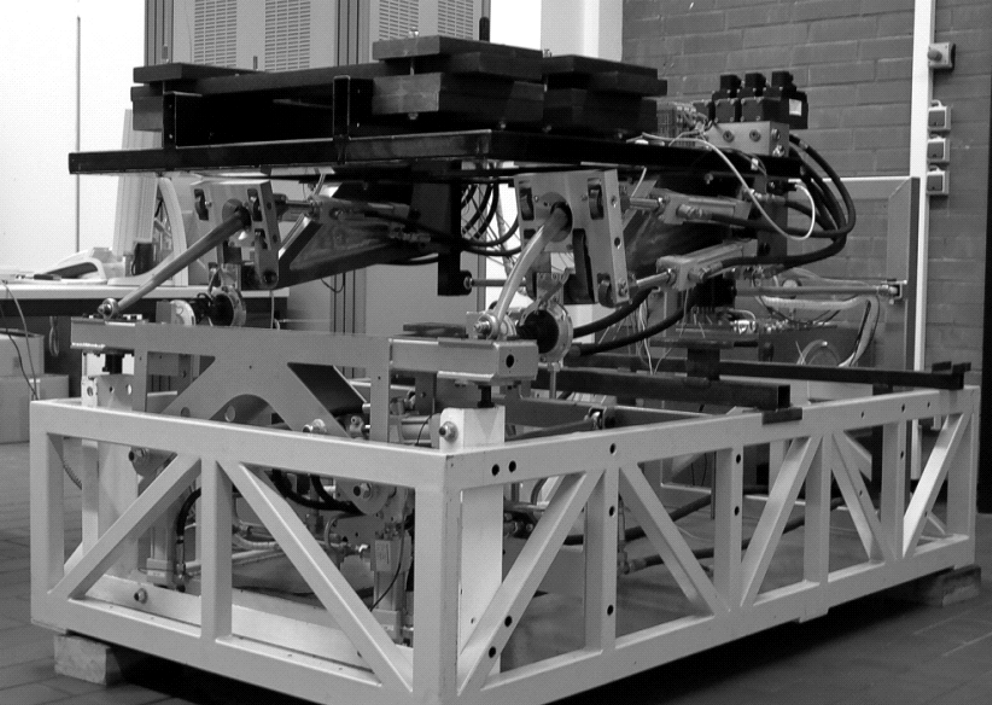
\includegraphics[width=0.7\textwidth]{Bilder/kapitel1/Pruefstand_Foto}
	\caption{Der SUrF-Prüfstand steht in unserem Labor, besteht aus ganz vielen Einzelteilen und ist ein spannendes Forschungsobjekt, vor allem aber ist dies nun eine Bildunterschrift über mehrere Zeilen.}
	\label{fig:surf}
\end{figure}

Beim Einbinden der Grafiken sollten absolute Pfade (C:/Dokumente und Einstellungen/ ... /Arbeit/Doku/Bilder/Bild1.pdf) vermieden werden. TeX kann mit relativen Pfaden umgehen (Bilder/Bild1.pdf). Damit ist sichergestellt, dass das Dokument jederzeit auch auf einem anderen Computer erstellt werden kann. Es kann sogar der Pfad eingestellt werden, in dem nach Grafiken gesucht wird. Dies geschieht in der Präambel mit \begin{lstlisting}[style=myLatexStyle]
	\graphicspath{{Bilder/kapitel1/},{...}}
\end{lstlisting}


Eine sehr schöne Möglichkeit um z.B. Matlab-Plots zu integrieren ist es, das \fe{pgfplots}-Package in Kombination mit der Matlabfunktion \fe{Matlab2tikz} (s. Dokumentenverzeichnis) zu verwenden. Dabei wird die figure in Matlab durch Aufrufen von 

ea\begin{lstlisting}[style=Matlab-editor]
	matlab2tikz('dateiname','width','\figurewidth','height','\figureheight')
\end{lstlisting}
 in eine \fe{.tex}-Datei mit den Dateinamen \fe{dateiname} und eine gespeichert. Sowohl die Text- als auch die Bildinformationen werden in der \fe{tex}-Datei hinterlegt und können mit einem Texeditor bearbeitet werden. Die Dateien können anschließend an passender Stelle mit dem Befehl \fe{$\backslash$ inserttikz} eingefügt werden. Die Befehlsreferenz
\begin{lstlisting}[style=myLatexStyle]
	\inserttikz{pfad/dateiname}{label}{caption}{Höhe}{Breite}{Pos}
	z.B 
	\inserttikz{Bilder/kapitel1/bspbild}{labeltest}{Testbild}{0.5\textwidth}{0.75\textwidth}{htbp}
\end{lstlisting}
führt auf das in Bild \ref{fig:gross} dargestellte Ergebnis. Möchte man das Bild nun verkleinert darstellen (s. \ref{fig:klein}) bleiben die Beschriftungen im passenden Schrifttyp und -größe.

\inserttikz{Bilder/kapitel1/bspbild}{fig:gross}{Bild wurde in Matlab generiert und mit \fe{matlab2tikz} exportiert}{0.4\textwidth}{0.7\textwidth}{htbp}

\inserttikz{Bilder/kapitel1/bspbild}{fig:klein}{Verkleinerte Version des zuvor eingefügten Bildes. Die Beschriftungen bleiben dennoch in einer leserlichen Größe}{0.2\textwidth}{0.5\textwidth}{htbp}
\clearpage
\subsection{Gleichungen}
Manchmal ist es aber mit Text nicht getan, dann ist unter Umständen eine Formel besser. Aber Achtung, Formeln sollten immer in den Text eingebunden werden und niemals für sich alleine stehen. Beispielsweise beschreiben die beiden Gleichungen 
\begin{es}
\label{eq:LTIsys} 
\dot{\vec{x}}(t) &= \vec{A}\vec{x}(t) + \vec{B}\vec{u}(t) \\
\vec{y}(t) &= \vec{C} \vec{x}(t)
\end{es}

mit	\begin{es}
	A & = ...\\
	B & = ...\\
	...
	\end{es}
ein lineares dynamisches System. Vektoren und Matrizen sollten mit dem Befehl \fe{\textbackslash vec\{\}} markiert werden. Die Gleichung \eqref{eq:LTIsys} ist außerdem ein Beispiel dafür, dass beide Gleichungen nur eine gemeinsame Formelnummer besitzen. Es bietet sich dafür an die Umgebung \fe{es} dafür benutzt werden. Es handelt sich dabei eine Kombination aus den Umgebungen \fe{align} und \fe{equation}.

Erst wenn man Gleichung \eqref{eq:LTIsys} mit \fe{eqref} referenziert, wird diese nummeriert! Dadurch wird vermieden, dass der Formelzähler unnötig groß wird.

Steht eine Formel am Ende eines Satzes, so ist ein Punkt innerhalb der Formelumgebung zu setzen, beispielsweise bei dieser Formel
\begin{equation}  
\label{eq:RiccatiJ}
J(x(t), u(t)) = \frac{1}{2} \int_0^\infty x(t)^T Q x(t) + u(t)^T S u(t) \ dt. 
\end{equation}
Hier beginnt dann ganz korrekt der neue Satz. Da auch die Gleichung \eqref{eq:RiccatiJ} eine wichtige Gleichung ist, die noch einmal referenziert wird, besitzt sie eine Formelnummer.

Mitunter muss man sogar Matrizen in der Arbeit angeben. Dazu ist es ganz praktikabel entsprechende Befehle zu verwenden und nicht selbst irgendetwas zusammen zu bauen. Es gibt sowohl Matrizen mit eckigen Klammer
\begin{equation}
\begin{bmatrix} A_{11} & A_{12} \\ A_{21} & A_{22} \end{bmatrix},
\end{equation}
als auch welche mit runden Klammern
\begin{equation*}
\begin{pmatrix} A_{11} & A_{12} \\ A_{21} & A_{22} \end{pmatrix}.
\end{equation*}

Mitunter fällt einem dann ein, dass an manchen Stellen noch etwas zu verbessern ist, aber man hat gerade keine Zeit oder keine Lust. Damit man seinen Gedankenblitz dann nicht so schnell vergisst, kann man den Befehl \fe{todo\{\}} zur graphischen Hervorhebung benutzen:
\todo{Dieser Absatz muss noch viel besser werden!}


Wenn Zahlen und Einheiten benötigt werden sollte das Paket \fe{siunitx} benutzt werden. Es ist in diesem Dokument so konfiguriert, dass es bei Zahlen immer ein Komma verwendet. 

\begin{itemize}
	\item\text{Einheit und Zahl} 
	\begin{lstlisting}[style=myLatexStyle]
	g=\SI{9.81}{\meter\per\square\second}
	\end{lstlisting} produziert die Ausgabe $g=\SI{9.81}{\meter\per\square\second}$\\
	\item\text{nur Zahl} 
	\begin{lstlisting}[style=myLatexStyle]
	\num{9.81}
	\end{lstlisting} produziert die Ausgabe $\num{9.81}$\\
	\item\text{nur Einheit} 
	\begin{lstlisting}[style=myLatexStyle]
	\si{\meter\per\square\second}
	\end{lstlisting} produziert die Ausgabe $\si{\meter\per\square\second}$
\end{itemize}
	
\subsection{Beispieltabellen}
Ansehnliche Tabellen lassen sich mit \fe{tabularx} und \fe{booktabs} erstellen. Die jeweiligen Spaltenbreiten lassen sich prozentual festlegen. Verwendet man eine "X"-Spalte ist der automatische Zeilenumbruch aktiviert.

Der Latex-Code
\begin{lstlisting}[style=myLatexStyle]
	\begin{table}[htbp] \caption{Mechanische Parameter des Doppelpendels auf einem Wagen}\label{tab:bsp}
	\begin{tabularx}{\linewidth}{
	>{\setlength\hsize{0.5\hsize}}X% 1.Spalte
	>{\setlength\hsize{0.25\hsize}}X% 2.Spalte
	>{\setlength\hsize{0.25\hsize}}X% 3.Spalte
	} 
	\toprule
	& innerer Pendelarm & äußerer Pendelarm\\
	& $i=1$ & $i=2$ \\ 
	\midrule
	Länge $l_i$ [\si{\meter}] & \num{0.356} & \num{0.356} \\
	Abstand zum Schwerpunkt $a_i$ [\si{\meter}]& \num{0.18} & \num{0.148} \\
	Masse $m_i$ [\si{\kilogram}] & \num{0.775} & \num{0.654} \\
	Trägheitsmoment $J_i$ [\si{\newton\meter\square\second}] & \num{0.0224} &\num{0.0179} \\
	Dämpfungskonstante $d_i$ [\si{\meter}] & \num{0.005} & \num{0.005} \\ 
	\bottomrule
	\end{tabularx}
	\end{table}
\end{lstlisting}
produziert die Tabelle \ref{tab:bsp}
\begin{table}[htbp] \caption{Mechanische Parameter des Doppelpendels auf einem Wagen}\label{tab:bsp}
	\begin{tabularx}{\linewidth}{
			>{\setlength\hsize{0.4\hsize}}X% 1.Spalte
			>{\setlength\hsize{0.3\hsize}}X% 2.Spalte
			>{\setlength\hsize{0.3\hsize}}X% 3.Spalte
		} 
		\toprule
		& innerer Pendelarm & äußerer Pendelarm\\
		& $i=1$ & $i=2$ \\ 
		\midrule
		Länge $l_i$ [\si{\meter}] & \num{0.356} & \num{0.356} \\
		Abstand zum Schwerpunkt $a_i$ [\si{\meter}]& \num{0.18} & \num{0.148} \\
		Masse $m_i$ [\si{\kilogram}] & \num{0.775} & \num{0.654} \\
		Trägheitsmoment $J_i$ [\si{\newton\meter\square\second}] & \num{0.0224} &\num{0.0179} \\
		Dämpfungskonstante $d_i$ [\si{\meter}] & \num{0.005} & \num{0.005} \\ 
		\bottomrule
	\end{tabularx}
\end{table}
%\include{Kapitel/kapitel2}						% in der Datei "gliederung.tex" (zu finden im Unterordner "Inhalt" im Root-Ordner) die Inhaltskapitel einbinden

	
	%%%%%%%%%%%%%%%%%%%%%%%%%%%%%%%%%%%%%%%%%%%%%%%%%%%%%%%%%%%%%%
	%  Literaturverzeichnis
	%%%%%%%%%%%%%%%%%%%%%%%%%%%%%%%%%%%%%%%%%%%%%%%%%%%%%%%%%%%%%%

	\newpage
	\cleardoublepage
	\bibliography{literatur}						% Erzeugung des Literaturverzeichnisses	
	\protect\thispagestyle{empty}					% auf dieser Seite keine Kopfzeile
	
	%%%%%%%%%%%%%%%%%%%%%%%%%%%%%%%%%%%%%%%%%%%%%%%%%%%%%%%%%%%%%%
	%  Anhang
	%%%%%%%%%%%%%%%%%%%%%%%%%%%%%%%%%%%%%%%%%%%%%%%%%%%%%%%%%%%%%%
	\cleardoublepage
	\protect\pagestyle{empty}						% auf den folgenden Seiten keine Kopfzeile
	\appendix
	\renewcommand{\thechapter}{A\arabic{chapter}}
	\renewcommand{\thefigure}{A\arabic{chapter}-\arabic{figure}}
	\renewcommand{\thetable}{A\arabic{chapter}-\arabic{table}}
	
	\cleardoublepage
	\addtocontents{toc}{\vspace*{2\baselineskip}}		% Abstand im Inhaltsverzeichnis vor Anhang
	\addtocontents{toc}{\protect\section*{Anhang}}		% erzeugt Anhangsverzeichnis nach dem Inhaltsverzeichnis
	\addtocontents{toc}{\vspace*{-0.2\baselineskip}}	% Abstand im Inhaltsverzeichnis nach Anhang
	
	\begingroup
	\let\clearpage\relax
	\chapter*{Anhang}
	\sffamily\listoftoc[Inhaltsverzeichnis]{toa}
	\endgroup
	\thispagestyle{empty}
	\cleardoublepage
	\lohead{Anhang~\headmark}
	\rehead{Anhang}			%
	\setcounter{page}{1}								% Seitenzahl auf 1 zurücksetzen
	\renewcommand{\thepage}{A-\arabic{page}}			% Seite im Anhang mit "A-XY"	
	 % !TeX encoding = UTF-8	
%%%%%%%%%%%%%%%%%%%%%%%%%%%%%%%%%%%%%%%%%%%%%%%%%%%%%%%%%%%%%%
%  Datenblätter
%%%%%%%%%%%%%%%%%%%%%%%%%%%%%%%%%%%%%%%%%%%%%%%%%%%%%%%%%%%%%%
\chapteranhang{Datenblätter}
%\datenblatt{sectionTitle}{filename}{seite}{caption}{refkey}
\datenblatt{Linearmotor}{linearmotor}{10}{Beispielhaftes Datenblatt eines Linearmotors der Firma Bosch/Rexroth}{anh:linearmotor}

%%%%%%%%%%%%%%%%%%%%%%%%%%%%%%%%%%%%%%%%%%%%%%%%%%%%%%%%%%%%%%
%  Zusätzliche Messungen
%%%%%%%%%%%%%%%%%%%%%%%%%%%%%%%%%%%%%%%%%%%%%%%%%%%%%%%%%%%%%%
\chapteranhang{Messungen}
%\messung{sectionTitle}{filename}{caption}{refkey}
\messung{Beispielmessung}{kapitel1/bspbild}{Messung im Anhang}{fig:beispielmessung}

							% in der Datei "anhang.tex" (zu finden im Unterordner "Inhalt" im Root-Ordner) die Anhänge einbinden
\end{document}
